% 模型的分析与检验（精简版：正文仅保留检验契约汇总表；其余 6 表与 1 图的环境移至文末"附录图表"块，排版时请移入正式附录，正文 \ref 编号不变）
\section{模型的分析与检验}

为检验结论的可信度及其成立条件，本章从灵敏度分析与模型检验两个层面展开验证：灵敏度分析通过对由数据估计或人为设定的关键参数施加合理扰动，考察最优决策与目标值是否发生量级性变化 \cite{saltelli2008}；模型检验则从分布诊断、样本外回测、基线对比、随机模拟与求解器状态校验等方面，检验模型假设、估计精度与求解可靠性。所有判定阈值均在运行前声明，检验契约（claim--perturbation--metric--threshold--observed--status）固化于 \texttt{q2\_robustness\_summary.json}，状态取 PASS 或 CONDITIONAL（边界在正文注明）；数值均可追溯至对应 CSV 与脚本（\texttt{A.py}--\texttt{D.py}、\texttt{q2\_sensitivity.py}、\texttt{q3.py}），随机模拟固定种子 SEED=7、每组样本量 $N=20000$，以保证可复现性。量级稳定判据为：利润与补货量扰动分别不超过 30\% 与 20\%，回测 MAPE 不超过 40\%，相关模拟期望利润偏差不超过 1\%。

\subsection{灵敏度分析}

\subsubsection{问题一：网络阈值与聚类稳定性}

相关系数阈值取 0.3、0.4、0.5 时，主边数分别为 1848、1062、523 条，稳健边数分别为 249、154、81 条（表~\ref{tab:threshold}，见附录），边数随阈值单调下降、正负边占比方向稳定，表明“品类/单品间以正相关为主、少数负相关”的结构性结论不依赖于阈值选择；主口径 0.4 下 154 条稳健边构成 51 节点协同变动网络。聚类簇数扫描中，silhouette 系数在 $k=5$ 处取得最大值 0.2583，超过 0.15 的选取下限（表~\ref{tab:silhouette}，见附录）；对 132 个单品做 80\% 抽样并重复聚类 50 次 \cite{efron1993}，平均调整兰德指数 ARI=0.4567，聚类结构中等稳定，且聚类标签与全样本独立重算的 Ward 聚类完全一致（特征最大偏差约 $10^{-14}$）。

\subsubsection{问题二：定价与补货参数灵敏度}

对批发价、价格弹性、价格口径与损耗率四类关键输入施加扰动，统一以未来一周总补货量与总期望利润为口径（表~\ref{tab:q2_sensitivity}、图~\ref{fig:q2_sensitivity}，见附录）：

\begin{itemize}
    \item \textbf{批发价 $\pm10\%$}：总补货量变化约 $\pm5\%$，总利润变化 +0.3\%/−0.7\%，均小于 1\%，定价与补货策略稳健（PASS）；
    \item \textbf{弹性 $\pm20\%$}：各品类弹性绝对值在 $\pm20\%$ 扰动后最大约 0.60，最优加价率与售价保持不变，总利润变化 −0.4\%/+0.5\%（PASS）；
    \item \textbf{价格口径切换}：当期销售额加权口径下弹性符号不变、绝对值普遍增大，利润 +26.7\%，与主口径机制一致；中位价口径下水生根茎类、食用菌弹性符号翻转、利润虚高 +72.8\%，该口径不可采用（CONDITIONAL）；
    \item \textbf{损耗率替换}：以 2022-07 至 2023-06 单品销量份额加权损耗率替代固定基期份额 $L_c=\sum_i w_i L_i$，利润 +7.5\%、补货量 −1.0\%，量级不变（PASS）。
\end{itemize}

\subsubsection{问题三：组合优化灵敏度}

对缺货惩罚、选品数、弹性、批发价、损耗率、价格网格与大 M 七类设定逐一重解 MIP（表~\ref{tab:q3_sensitivity}，见附录），全部情景求解状态 optimal、最优性 gap=0。缺货惩罚 $\rho$（0.5--1.5）与大 M 放大 50\% 情景的最优解完全不变：前者因基准方案无缺货、惩罚项不进入目标值，后者结合订购量上界余量检查（最小余量 12.58 kg）确认可行域未被截断。选品数 27/30/33 对应利润 657.54/673.60/682.08 元；弹性 $\pm20\%$ 使利润变化 −1.6\%/+1.7\%，方向与问题二一致；批发价 $\pm10\%$ 为最敏感输入（利润 −17.6\%/+18.1\%），且 $\times1.1$ 时 1 个低毛利单品被挤出；损耗率取分类级时利润 −3.6\%；价格网格 $K=7$ 与分位数取点分别使利润 −3.7\%/+4.5\%，离散化影响控制在 $\pm5\%$ 以内。

\subsection{模型检验与误差分析}

\subsubsection{问题一：分布、季节与关联结构检验}

六品类日销量按 AIC 选型为伽马（4 个）与对数正态（2 个），BIC 交叉核对一致，QQ 图无系统性偏离（图~\ref{fig:dist_qq}）；K-S 检验在参数估计后偏保守，仅作图形诊断。STL 分解的季节强度 0.1729--0.2616、趋势强度 0.5135--0.6268，与独立重算最大偏差 $5\times10^{-5}$。协同网络主边 1062 条中 154 条通过前后半样本检验成为稳健边，抽样 200 条边独立重算的相关系数最大偏差 $5\times10^{-5}$，FDR $q$ 值与标准 BH 校正一致；聚类抽样稳定性 ARI=0.4567（见 9.1.1）。

\subsubsection{问题二：需求—价格模型、预测与报童检验}

回归诊断表明，六品类价格弹性 $t$ 值分别为 −6.79、−5.45、−0.70、−3.16、−3.03、−5.28，除水生根茎类（$t=-0.70$）外均在 1\% 水平显著，该品类定价结论相应降级（详见表~\ref{tab:q2_elasticity}）；$R^2$ 介于 0.31--0.61，$\ln P$ 相关矩阵条件数为 7.9，不存在严重共线性（图~\ref{fig:q2_elasticity}）。

样本外回测以 MAPE 度量，求和仅对实际销量 $Q_t>0$ 的日期进行：
\begin{equation}
\mathrm{MAPE}=\frac{100\%}{n}\sum_{t}\frac{\left|\hat Q_t-Q_t\right|}{Q_t}.
\end{equation}
后 28 天滚动回测 MAPE 为 20.6\%--37.2\%；2022-07 同期回测为 23.9\%--66.4\%，除辣椒类外各品类误差均高于后 28 天口径，最大 66.4\%（茄类）超过 40\% 阈值（CONDITIONAL），表明跨年外推稳定性有限，2023-07 预测区间应保守解读（表~\ref{tab:backtest}，见附录；数据文件：\texttt{q2\_backtest.csv}、\texttt{q2\_backtest\_2022.csv}）。

基线对比中，报童最优分位数订货相对确定性补货 $R^0_{c,t}=\mu_{c,t}(P^*)/(1-L_c)$ 的总期望利润为 5305.19 vs 4550.45 元（增益 +754.74 元），总补货量 2607.89 vs 3190.54 kg（低 18.3\%），日均缺货率 0.51--0.80 vs 0.39--0.43，体现“少订少损耗换更高期望利润”的最优取舍；水生根茎类在确定性口径下利润为负（−112.79 元）、报童口径转正（360.99 元），与其临界比最小（$\kappa=0.20$）一致（表~\ref{tab:nv_det}，见附录；数据文件：\texttt{q2\_nv\_det.csv}）\cite{han2026}。

品类相关联合模拟以残差 Pearson 相关矩阵（非对角元 0.24--0.74）构造高斯 copula \cite{nelsen2006}，配合对数正态边际模拟每日 2 万组（SEED=7）：相关口径期望利润 5311.26 vs 独立口径 5305.19 元（+0.11\%，在 1\% 阈值内，PASS），方差比 2.47，证实“相关性只进入方差、不进期望”（数据文件：\texttt{q2\_joint\_sim.csv}）。

\subsubsection{问题三：求解可靠性与可行性检验}

基准及全部灵敏度情景求解状态 status=0、最优性 gap=0，五项约束逐条校验通过（选品数 33 $\in$ [27,33]、最小陈列量 2.5 kg、可售量 $\le$ 订购量 $\times(1-L_i)$、价格在网格内、品类全覆盖）（数据文件：\texttt{q3\_diagnostics.csv}）；3 个低需求单品因最小陈列约束超订 1.16 kg（成本 10.53 元）已计入成本。大 M 取值 $\max(3\max_t Q_{i,t}^{\mathrm{hist}},\ 2.5,\ 1.05D_{i,1})$ 的最小余量 12.58 kg，放大 50\% 后最优解不变，双重确认可行域未被截断（数据文件：\texttt{q3\_mbound.csv}）。跨问题交叉核对中，问题三各品类可售量加总 $\sum_{i\in\mathcal{C}_c}q_i(1-L_i)$ 与问题二品类期望需求 $\mu_{c,t}(P^*)$ 之比为 0.21--0.74，量级同阶、结构一致，差异源于计划层级与约束口径，属预期差异而非矛盾（数据文件：\texttt{q3\_vs\_q2.csv}）。

\subsubsection{检验结论汇总}

七项量化检验的契约见表~\ref{tab:summary}：5 项 PASS、2 项 CONDITIONAL（中位价口径不可采用、2022-07 跨年回测误差更高），相应边界已在正文标注；主结论在参数扰动、口径替换、基线对比与随机模拟下保持稳健。

\begin{table}[htbp]
\centering
\caption{模型检验契约汇总（阈值运行前声明）}
\label{tab:summary}
\begin{tabular}{l l r r l}
\toprule
检验项 & 扰动/方法 & 阈值 & 观测值 & 状态 \\
\midrule
批发价 $\pm10\%$ 利润稳定 & $W\times1.1$、$W\times0.9$ & $\le30\%$ & 0.7\% & PASS \\
弹性 $\pm20\%$ 决策稳定 & 品类弹性 $\times1.2$、$\times0.8$ & $\le30\%$ & 0.5\% & PASS \\
价格口径切换 & 固定权重→当期加权/中位价 & $\le30\%$ & 72.8\% & CONDITIONAL \\
报童优于确定性 & 最优分位数 $y^*$ vs 均值 & 利润差 $\ge0$ & +754.74 元 & PASS \\
损耗率替换 & 固定份额→单品销量加权 & 补货变化 $\le20\%$ & 1.0\%（补货量） & PASS \\
2022-07 同期回测 & 样本截止 2022-06-30 & MAPE $\le40\%$ & 66.4\% & CONDITIONAL \\
品类相关联合模拟 & 残差相关 vs 独立（高斯 copula） & 利润偏差 $\le1\%$ & 0.11\% & PASS \\
\bottomrule
\end{tabular}
\end{table}

\subsubsection{模型局限（三问共享）}

缺货日销量截断使需求与弹性估计轻微低估；水生根茎类弹性不显著（$t=-0.70$），其定价结论证据不足；跨年（2022-07）预测误差高于后 28 天口径，外推至 2023-07 应保守。

\subsection*{本章小结}

三问结论在灵敏度与模型检验下量级稳定：问题一结构结论不依赖阈值选择、聚类 ARI=0.4567；问题二批发价与弹性扰动下利润变化均小于 1\%，报童增益 +754.74 元，相关模拟证实“相关性只进入方差、不进期望”（偏差 +0.11\%，方差比 2.47）；问题三全部情景 optimal 且约束通过，批发价为最敏感输入（约 $\pm18\%$）、网格离散化影响约 $\pm4.5\%$。七项检验 5 项 PASS、2 项 CONDITIONAL，在标注的两项边界条件下，模型结论可作为商超补货定价决策的依据。

%% ===================== 附录图表（排版时请移入正式附录；正文引用编号不变） =====================

\begin{table}[htbp]
\centering
\caption{相关系数阈值敏感性（数据文件：\texttt{q1\_corr\_threshold.csv}）}
\label{tab:threshold}
\begin{tabular}{c r r r r}
\toprule
阈值 & 主边数 & 正边数 & 负边数 & 稳健边数 \\
\midrule
0.3 & 1848 & 1289 & 559 & 249 \\
0.4 & 1062 & 820  & 242 & 154 \\
0.5 & 523  & 456  & 67  & 81  \\
\bottomrule
\end{tabular}
\end{table}

\begin{table}[htbp]
\centering
\caption{层次聚类候选 $k$ 的 silhouette 系数（数据文件：\texttt{q1\_cluster\_k.csv}）}
\label{tab:silhouette}
\begin{tabular}{c c c c c c c c c}
\toprule
候选 $k$ & 3 & 4 & 5 & 6 & 7 & 8 & 9 & 10 \\
\midrule
silhouette & 0.2083 & 0.2429 & \textbf{0.2583} & 0.2579 & 0.2192 & 0.2257 & 0.2269 & 0.2058 \\
稳定性 ARI & --- & --- & 0.4567 & --- & --- & --- & --- & --- \\
\bottomrule
\end{tabular}
\par\medskip\footnotesize 注：$k=5$ 与 $k=6$ 的 silhouette 接近（0.2583 与 0.2579），结合稳定性 ARI 与簇的可解释性取 $k=5$。
\end{table}

\begin{table}[htbp]
\centering
\caption{问题二灵敏度分析结果（基准：补货 2607.89 kg、利润 5305.19 元）}
\label{tab:q2_sensitivity}
\begin{tabular}{l r r r}
\toprule
情景 & 7 天总补货量（kg） & 7 天总利润（元） & 利润变化 \\
\midrule
基准 & 2607.89 & 5305.19 & --- \\
批发价 +10\% & 2490.69 & 5322.36 & +0.3\% \\
批发价 −10\% & 2733.33 & 5270.62 & −0.7\% \\
弹性 +20\% & 2608.90 & 5282.80 & −0.4\% \\
弹性 −20\% & 2608.79 & 5330.49 & +0.5\% \\
损耗率 = 单品销量加权 & 2582.87 & 5705.22 & +7.5\% \\
价格口径 = 当期销售额加权 & 2536.22 & 6722.15 & +26.7\% \\
价格口径 = 中位价 & 2801.29 & 9165.93 & +72.8\% \\
\bottomrule
\end{tabular}
\end{table}

\begin{figure}[htbp]
\centering
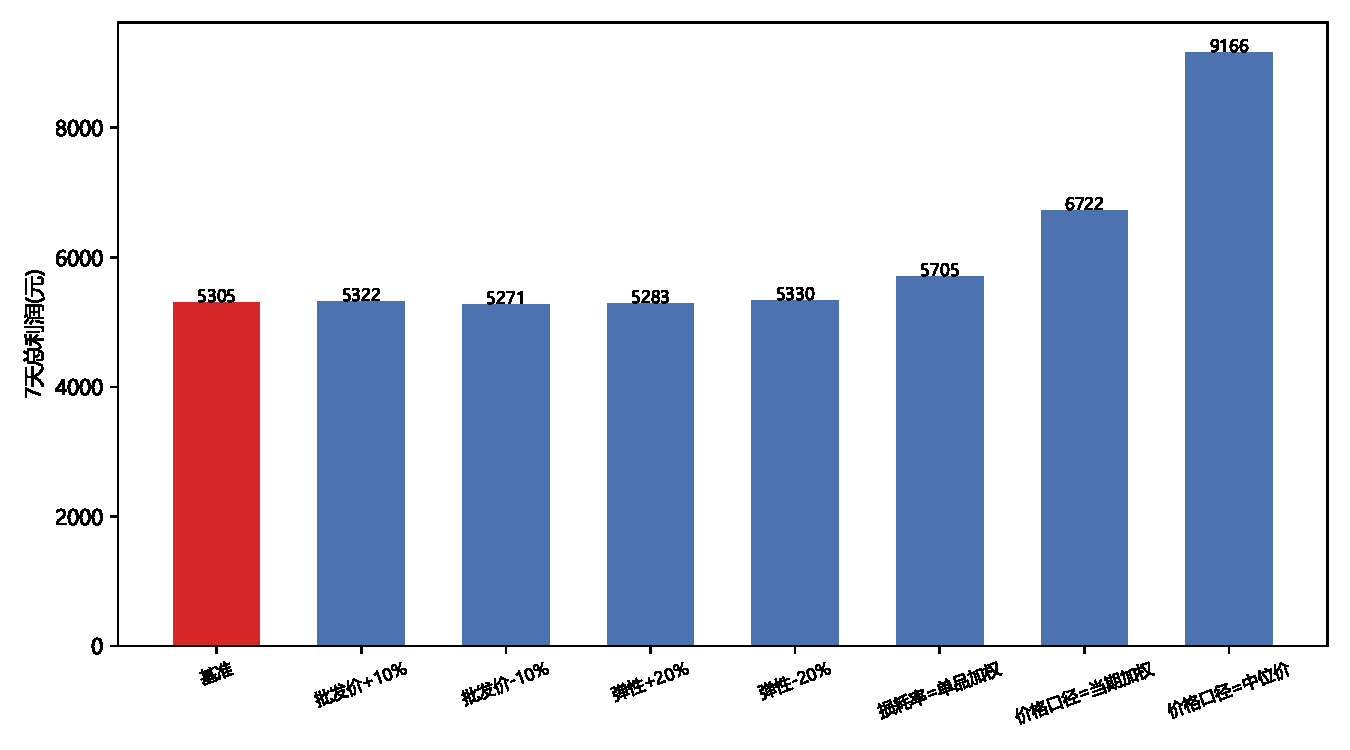
\includegraphics[width=0.8\linewidth]{figures/q2_sensitivity.pdf}
\caption{问题二各灵敏度情景下未来一周总期望利润对比（红色柱为基准情景）}
\label{fig:q2_sensitivity}
\end{figure}

\begin{table}[htbp]
\centering
\caption{问题三灵敏度分析结果（基准：利润 682.08 元、满足率 1.00、选中 33 个）}
\label{tab:q3_sensitivity}
\begin{tabular}{l r r r}
\toprule
情景 & 总利润（元） & 满足率 & 选中数 \\
\midrule
$\rho=0.5$   & 682.08 & 1.00 & 33 \\
$\rho=1.0$（基准） & 682.08 & 1.00 & 33 \\
$\rho=1.5$   & 682.08 & 1.00 & 33 \\
选品数 = 27 & 657.54 & 1.00 & 27 \\
选品数 = 30 & 673.60 & 1.00 & 30 \\
选品数 = 33 & 682.08 & 1.00 & 33 \\
弹性 $\times 1.2$ & 670.92 & 1.00 & 33 \\
弹性 $\times 0.8$ & 693.75 & 1.00 & 33 \\
批发价 $\times 1.1$ & 561.98 & 1.00 & 32 \\
批发价 $\times 0.9$ & 805.49 & 1.00 & 33 \\
损耗率 = 分类级 & 657.44 & 1.00 & 33 \\
网格 $K=7$ & 656.78 & 1.00 & 33 \\
网格 = 分位数取点 & 712.69 & 1.00 & 33 \\
大 M $\times 1.5$ & 682.08 & 1.00 & 33 \\
\bottomrule
\end{tabular}
\end{table}

\begin{table}[htbp]
\centering
\caption{预测回测 MAPE（\%）}
\label{tab:backtest}
\begin{tabular}{l r r}
\toprule
品类 & 后 28 天 MAPE & 2022-07 同期 MAPE \\
\midrule
花叶类 & 24.1 & 29.9 \\
花菜类 & 37.2 & 46.5 \\
水生根茎类 & 20.6 & 60.3 \\
茄类 & 30.3 & 66.4 \\
辣椒类 & 27.4 & 23.9 \\
食用菌 & 23.5 & 43.1 \\
\bottomrule
\end{tabular}
\end{table}

\begin{table}[htbp]
\centering
\caption{报童与确定性订货对比（未来一周，数据文件：\texttt{q2\_nv\_det.csv}）}
\label{tab:nv_det}
\begin{tabular}{l r r r r r r}
\toprule
品类 & 报童补货（kg） & 确定性补货（kg） & 补货降幅 & 报童利润（元） & 确定性利润（元） & 日均缺货率（报童/确定性） \\
\midrule
花叶类 & 1182.61 & 1338.92 & 11.7\% & 2517.33 & 2447.20 & 0.57/0.43 \\
花菜类 & 133.07 & 200.86 & 33.7\% & 355.93 & 230.06 & 0.69/0.39 \\
水生根茎类 & 175.91 & 332.03 & 47.0\% & 360.99 & −112.79 & 0.80/0.39 \\
茄类 & 157.01 & 188.19 & 16.6\% & 365.76 & 347.50 & 0.56/0.41 \\
辣椒类 & 540.64 & 595.51 & 9.2\% & 1209.04 & 1192.69 & 0.51/0.42 \\
食用菌 & 418.66 & 535.04 & 21.8\% & 496.14 & 445.79 & 0.61/0.41 \\
合计 & 2607.89 & 3190.54 & 18.3\% & 5305.19 & 4550.45 & --- \\
\bottomrule
\end{tabular}
\end{table}
